\documentclass[12pt]{article}

% packages

%\usepackage{times} % alt: cmbright
\usepackage[top=1in, bottom=1in, left=1in, right=1in]{geometry}
\usepackage{natbib}
\usepackage{amsmath}
\usepackage{amssymb}
\usepackage{latexsym}
\usepackage{sectsty}
\usepackage{amsfonts}
\usepackage{epsfig}
\usepackage{url}
\usepackage{microtype}
\usepackage{fixmath}
\usepackage{hyperref}
\usepackage{graphicx}

% references

\newcommand{\mysec}[1]{Section~\ref{sec:#1}}
\newcommand{\myapp}[1]{Appendix~\ref{app:#1}}
\newcommand{\myeq}[1]{Equation~\ref{eq:#1}}
\newcommand{\myeqp}[1]{Eq.~\ref{eq:#1}}
\newcommand{\mychap}[1]{Chapter~\ref{chap:#1}}
\newcommand{\myfig}[1]{Figure~\ref{fig:#1}}

% math conveniences

\newcommand{\g}{\,\vert\,}
\newcommand{\E}{\textrm{E}}
\newcommand{\vct}[1]{\textbf{#1}}
\newcommand{\realline}{\mathbb{R}}
\newcommand{\indpt}{\protect\mathpalette{\protect\independenT}{\perp}}
\def\independenT#1#2{\mathrel{\rlap{$#1#2$}\mkern2mu{#1#2}}}
\newcommand{\h}[1]{\textrm{H}\left( #1 \right)}
\newcommand{\half}{\frac{1}{2}}
\newcommand{\new}{\textrm{new}}

\newcommand{\mult}{\textrm{Mult}}
\newcommand{\dir}{\textrm{Dir}}
\newcommand{\discrete}{\textrm{Discrete}}
\newcommand{\Bern}{\textrm{Bern}}
\newcommand{\DP}{\textrm{DP}}
\newcommand{\GP}{\textrm{GP}}
\newcommand{\Bet}{\textrm{Beta}}

% paragraph spacing

\setlength{\parindent}{0pt}
\setlength{\parskip}{2ex plus 0.5ex minus 0.2ex}

\allsectionsfont{\sffamily\mdseries}
\paragraphfont{\sffamily\bfseries}


\usepackage{fontspec}
\setmainfont{WenQuanYi Zen Hei}

%\hbadness=10000
%\tolerance=10000
%\hfuzz=100pt


\begin{document}

\title{\textsf{A simple gibbs sampling example}}
\author{\textsf{lleia@qq.com}}
\date{\today}
\maketitle

\section{The Change Point Model}
This example can be found \href{http://www.bcs.rochester.edu/people/robbie/jacobslab/cheat_sheet/GibbsSampling.pdf}{here}. Since its simplicity, we can focus on the most important sampling part of the model instead of being lost in the mathematical details. The quotation below is the problem:

\begin{quotation}
Suppose that we observe a sequence of counts $x_1,x_2,\cdots,x_N$ where the average of the counts has some value for time steps from 1 to $n$, and a different value for time steps $n+1$ to $N$.
\end{quotation} 

We use poisson distributions to model the generating of the sequence and leverage a $\Gamma$ distribution for its priors.So for the first part of the sequence, we have a parameter $\lambda_1$ and every $x_i \sim poisson(\lambda_1)$ and so are the remains. Finally the model has been crafted:   

\begin{align}
	n & \sim   Uniform(1,2,\cdots,N) \\
	\lambda_i & \sim  \Gamma(\lambda;a,b) \\
	x_i & \sim  \begin{cases} Poisson(x;\lambda_1),i \le n\\ Poisson(x;\lambda_2), i > n \end{cases} \\
	p(X,n,\lambda_1,\lambda_2) &= p(n)p(\lambda_1)p(\lambda_2)p(X_{1,2,\cdots,n}|\lambda_1)p(X_{n+1,n+2,\cdots,N}|\lambda_2)
\end{align}

\section{Poisson Distribution and Gamma Distribution}\label{section:conjugate}
Suppose $p(\lambda) \sim \Gamma(\lambda;a,b)$, $p(x|\lambda) \sim Poisson(x;\lambda)$,now we calculate the $p(\lambda|x)$.

%calculate the posterior distribution
\begin{equation}
\begin{split}
p(\lambda|X) & = \frac{p(X|\lambda)p(\lambda)}{p(X)} \\
			 & \propto p(X|\lambda)p(\lambda) \\
			 & = \prod_{i=1}^N p(x_i|\lambda) p(\lambda) \\ 
			 & = \prod_{i=1}^N e^{-\lambda} \frac{\lambda^{x_i}}{x_i!} \frac{1}{\Gamma(a)}b^a\lambda^{a-1}e^{-b\lambda} \\
			 & = e^{-N\lambda}\frac{\lambda^{\sum_{i=1}^Nx_i}}{\prod_{i=1}^{N}x_i!}\frac{1}{\Gamma(a)}b^a\lambda^{a-1}e^{-b\lambda} \\
			 & = \frac{b^a}{\Gamma(a)\prod_{n=1}^Nx_i!}\lambda^{a+\sum_{i=1}^Nx_i-1}e^{-(b+N)\lambda} \\
			 & \propto \Gamma(\lambda;a+\sum_{i=1}^Nx_i,b+N)
\end{split}
\end{equation}
So the Gamma and Poisson are conjugate distributions.

\section{The Gibbs Sampler}
We now derive a gibbs sampler for the change point model. Note that we want to kown the posterior:
$$ p(n,\lambda_1,\lambda_2|X) $$
We need all the conditional distributions in order to run the gibbs sampler. For $p(n|\lambda_1,\lambda_2,X)$,
\begin{equation}\label{formula:npost} 
\begin{split}
p(n|\lambda_1,\lambda_2,X) & = \frac{p(n,\lambda_1,\lambda_2,X)}{p(\lambda_1,\lambda_2,X)} \\
						   & \propto p(n,\lambda_1,\lambda_2,X) \\
						   & = p(n) p(\lambda_1) p(\lambda_2) p(X_{1,2,\cdots,n}|\lambda_1) p(X_{n+1,n+2,\cdots,N}|\lambda_2) \\
						   & \propto p(X_{1,2,\cdots,n}|\lambda_1) p(X_{n+1,n+2,\cdots,N}|\lambda_2) \\ 
						   & = \prod_{i=1}^n e^{-\lambda_1}\frac{\lambda_1^{x_i}}{x_i!} \prod_{i=n+1}^N e^{-\lambda_2}\frac{\lambda_2^{x_i}}{x_i!} \\
						   & \propto \prod_{i=1}^n e^{-\lambda_1}\lambda_1^{x_i} \prod_{i=n+1}^N e^{-\lambda_2} \lambda_2^{x_i} \\
						   & = exp(-n\lambda_1 - (N-n)\lambda_2)\lambda_1^{\sum_{i=1}^nx_i}\lambda_2^{\sum_{i=n+1}^Nx_i} \\
						   & = exp(\sum_{i=1}^nx_ilog\lambda_1 + \sum_{i=n+1}^Nx_ilog\lambda_2 - n\lambda_1 - (N-n)\lambda_2) 
\end{split}
\end{equation}

So we sample $n$ from a multinomial distribution which depends on $\lambda_1$, $\lambda_2$. Since $p(\lambda_1|\lambda_2,n,X) \propto p(\lambda_1|X_{1,2,\cdots,n})$,just as in section \ref{section:conjugate}, we have:

\begin{equation}
\begin{split}
p(\lambda_1|\lambda_2,n,X) & \propto p(\lambda_1,\lambda_2,n,X) \\  
						   & \propto p(\lambda_1|X_{1,2,\cdots,n}) \\
						   & = \Gamma(\lambda_1;a + \sum_{i=1}^nX_i,b + n)
\end{split}
\end{equation}

$\lambda_2$ has the same story:
\begin{equation}
p(\lambda_2|\lambda_1,n,X) \propto \Gamma(\lambda_2; a + \sum_{i=n+1}^NX_i,b+(N-n))
\end{equation}

Put all these things together, we have the gibbs sampler for our problem as below:

\begin{algorithm}[H]
\KwData{observed sequence $x_1,x_2,\cdots,x_n$}
\KwResult{$n,\lambda_1,\lambda_2$}
$i = 1$\;
\While{the sampler has not converged} {
	sample $n_i \sim multinomial$ as in formula \ref{formula:npost}\;
	sample $\lambda_{i1} \sim \Gamma(a+\sum_{i=1}^nx_i,b+n_i)$\;
	sample $\lambda_{i2} \sim \Gamma(a+\sum_{i=n+1}^Nx_i,b+N-n_i)$\;
	$i = i + 1$\;
}
\caption{Gibbs Sampler}
\end{algorithm}

\section{Experiments}
Here is the r \href{https://github.com/lleia/miscelaneous/blob/master/r/change_point_model/changePointModel.r}{code}. We use two binomial distributions (with 10 and 30 as expection respectively) to generate a sequence of length 100. After 10000 iterations,we get results as below,as we can see from the pictures, the sampling results work well to fit our test sequence.
 
\begin{figure}
\caption{Test Sequence}
\centering
	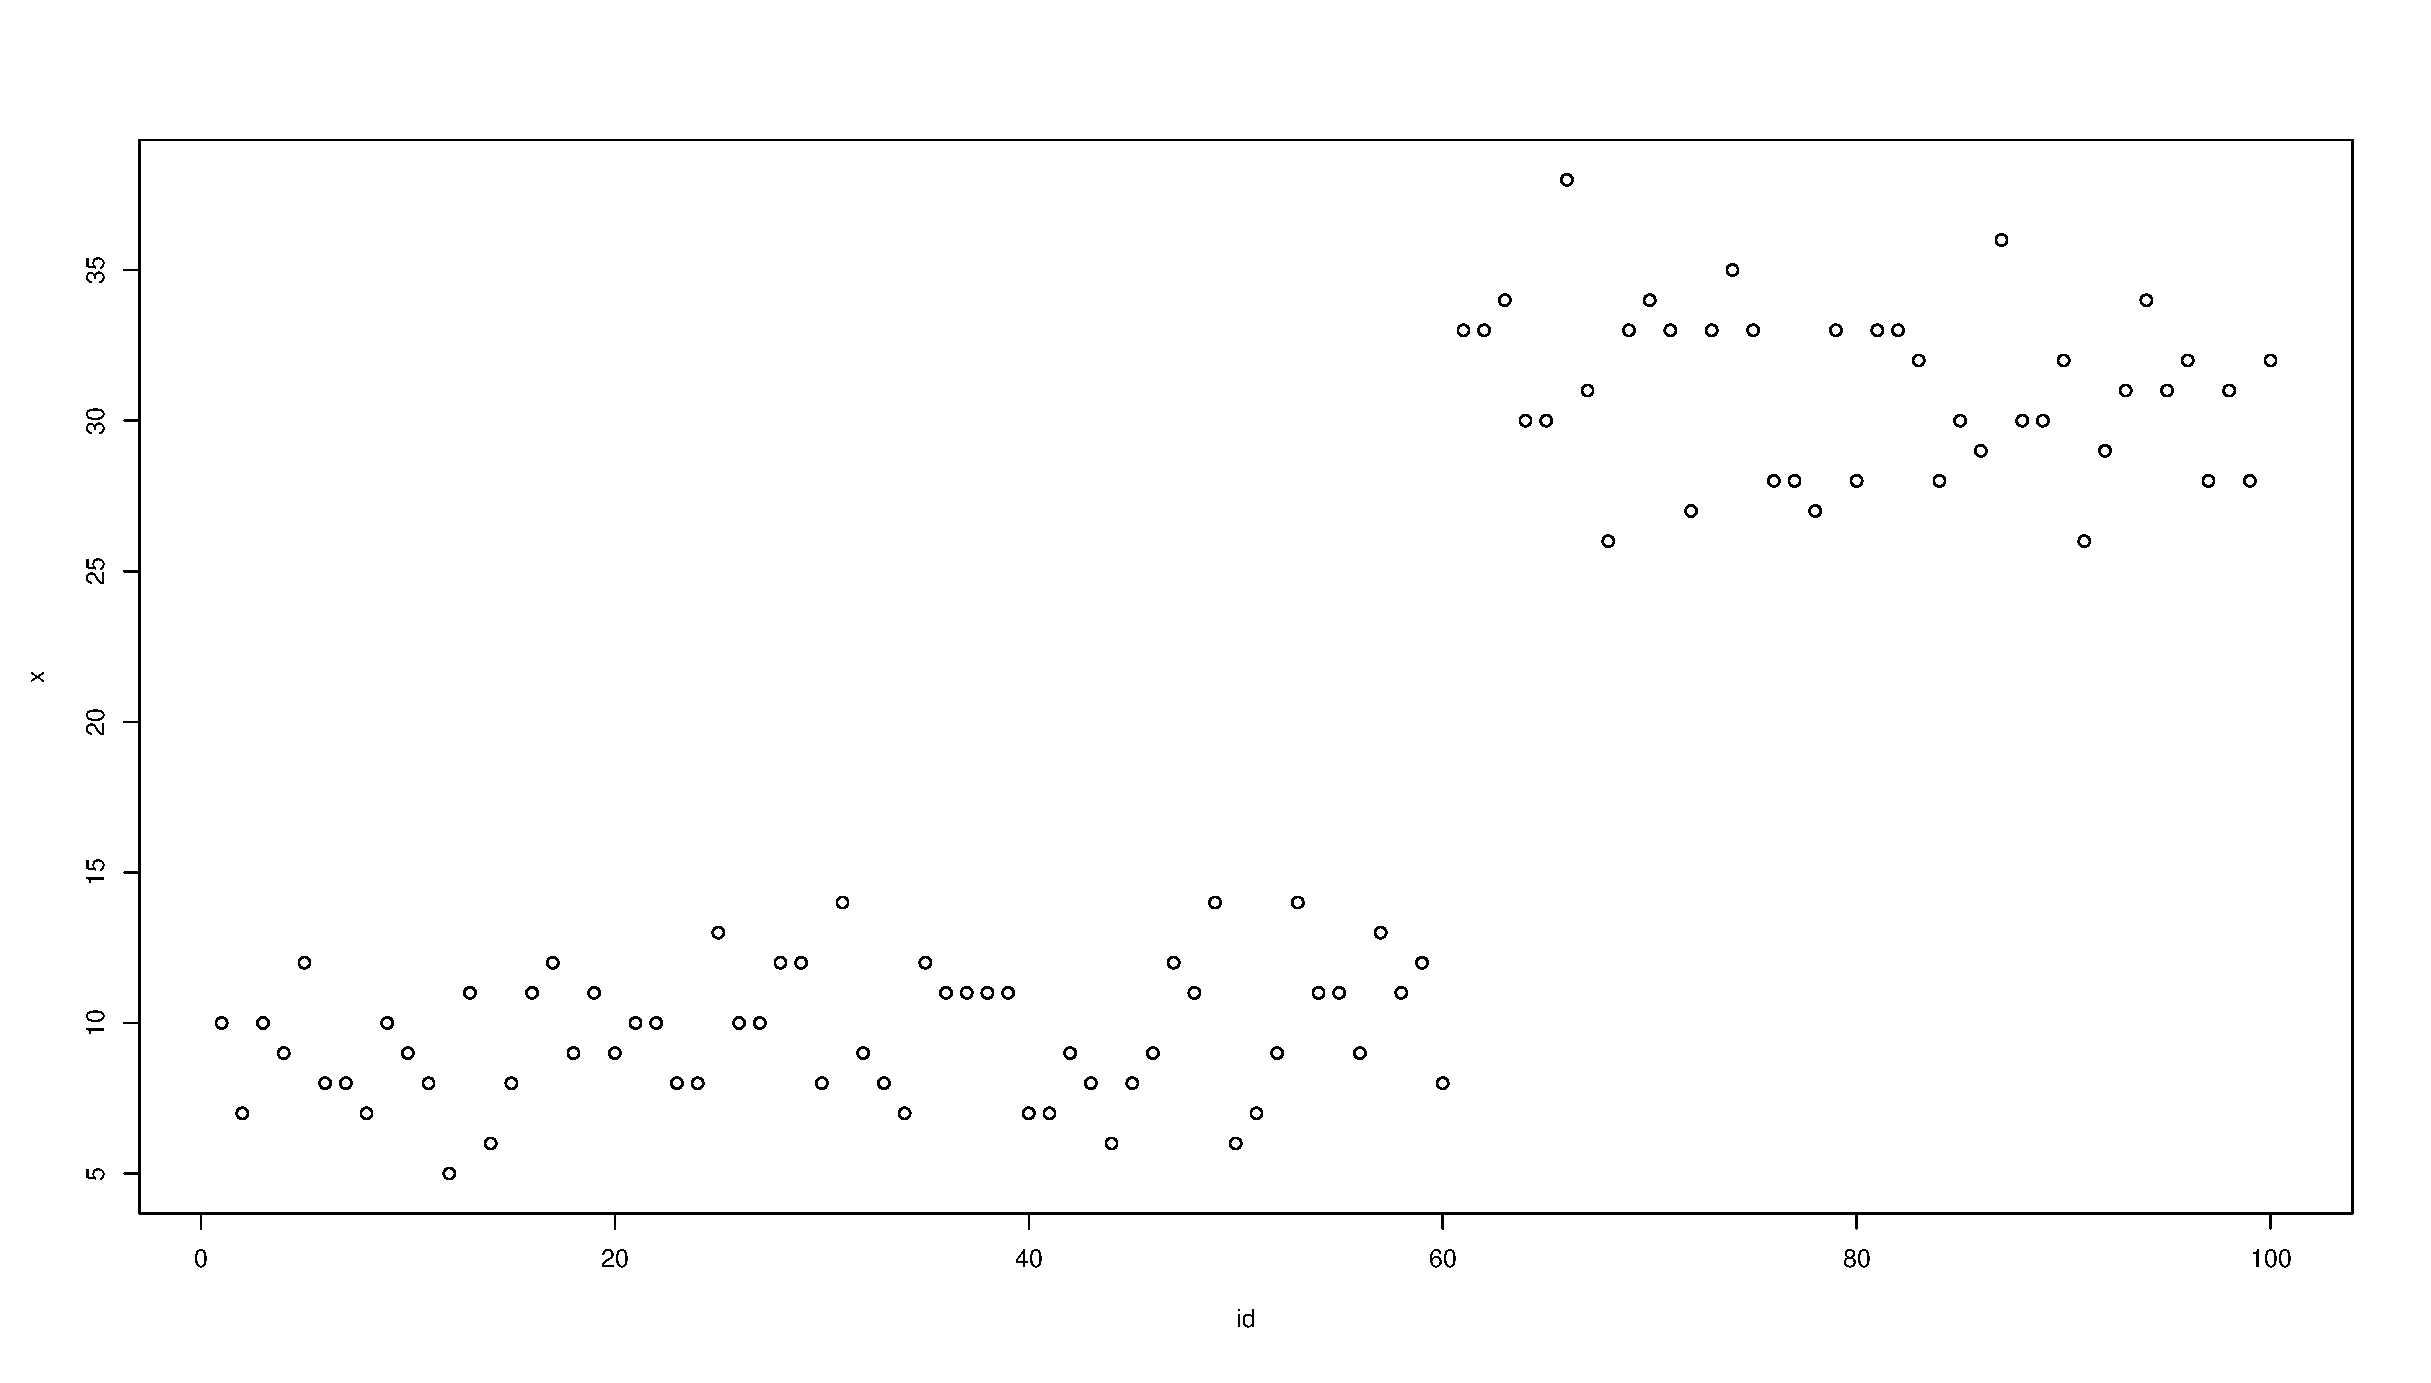
\includegraphics[width=5in]{seq.eps}
\end{figure}


\begin{figure}
\caption{Sampling of $n$}
\centering
	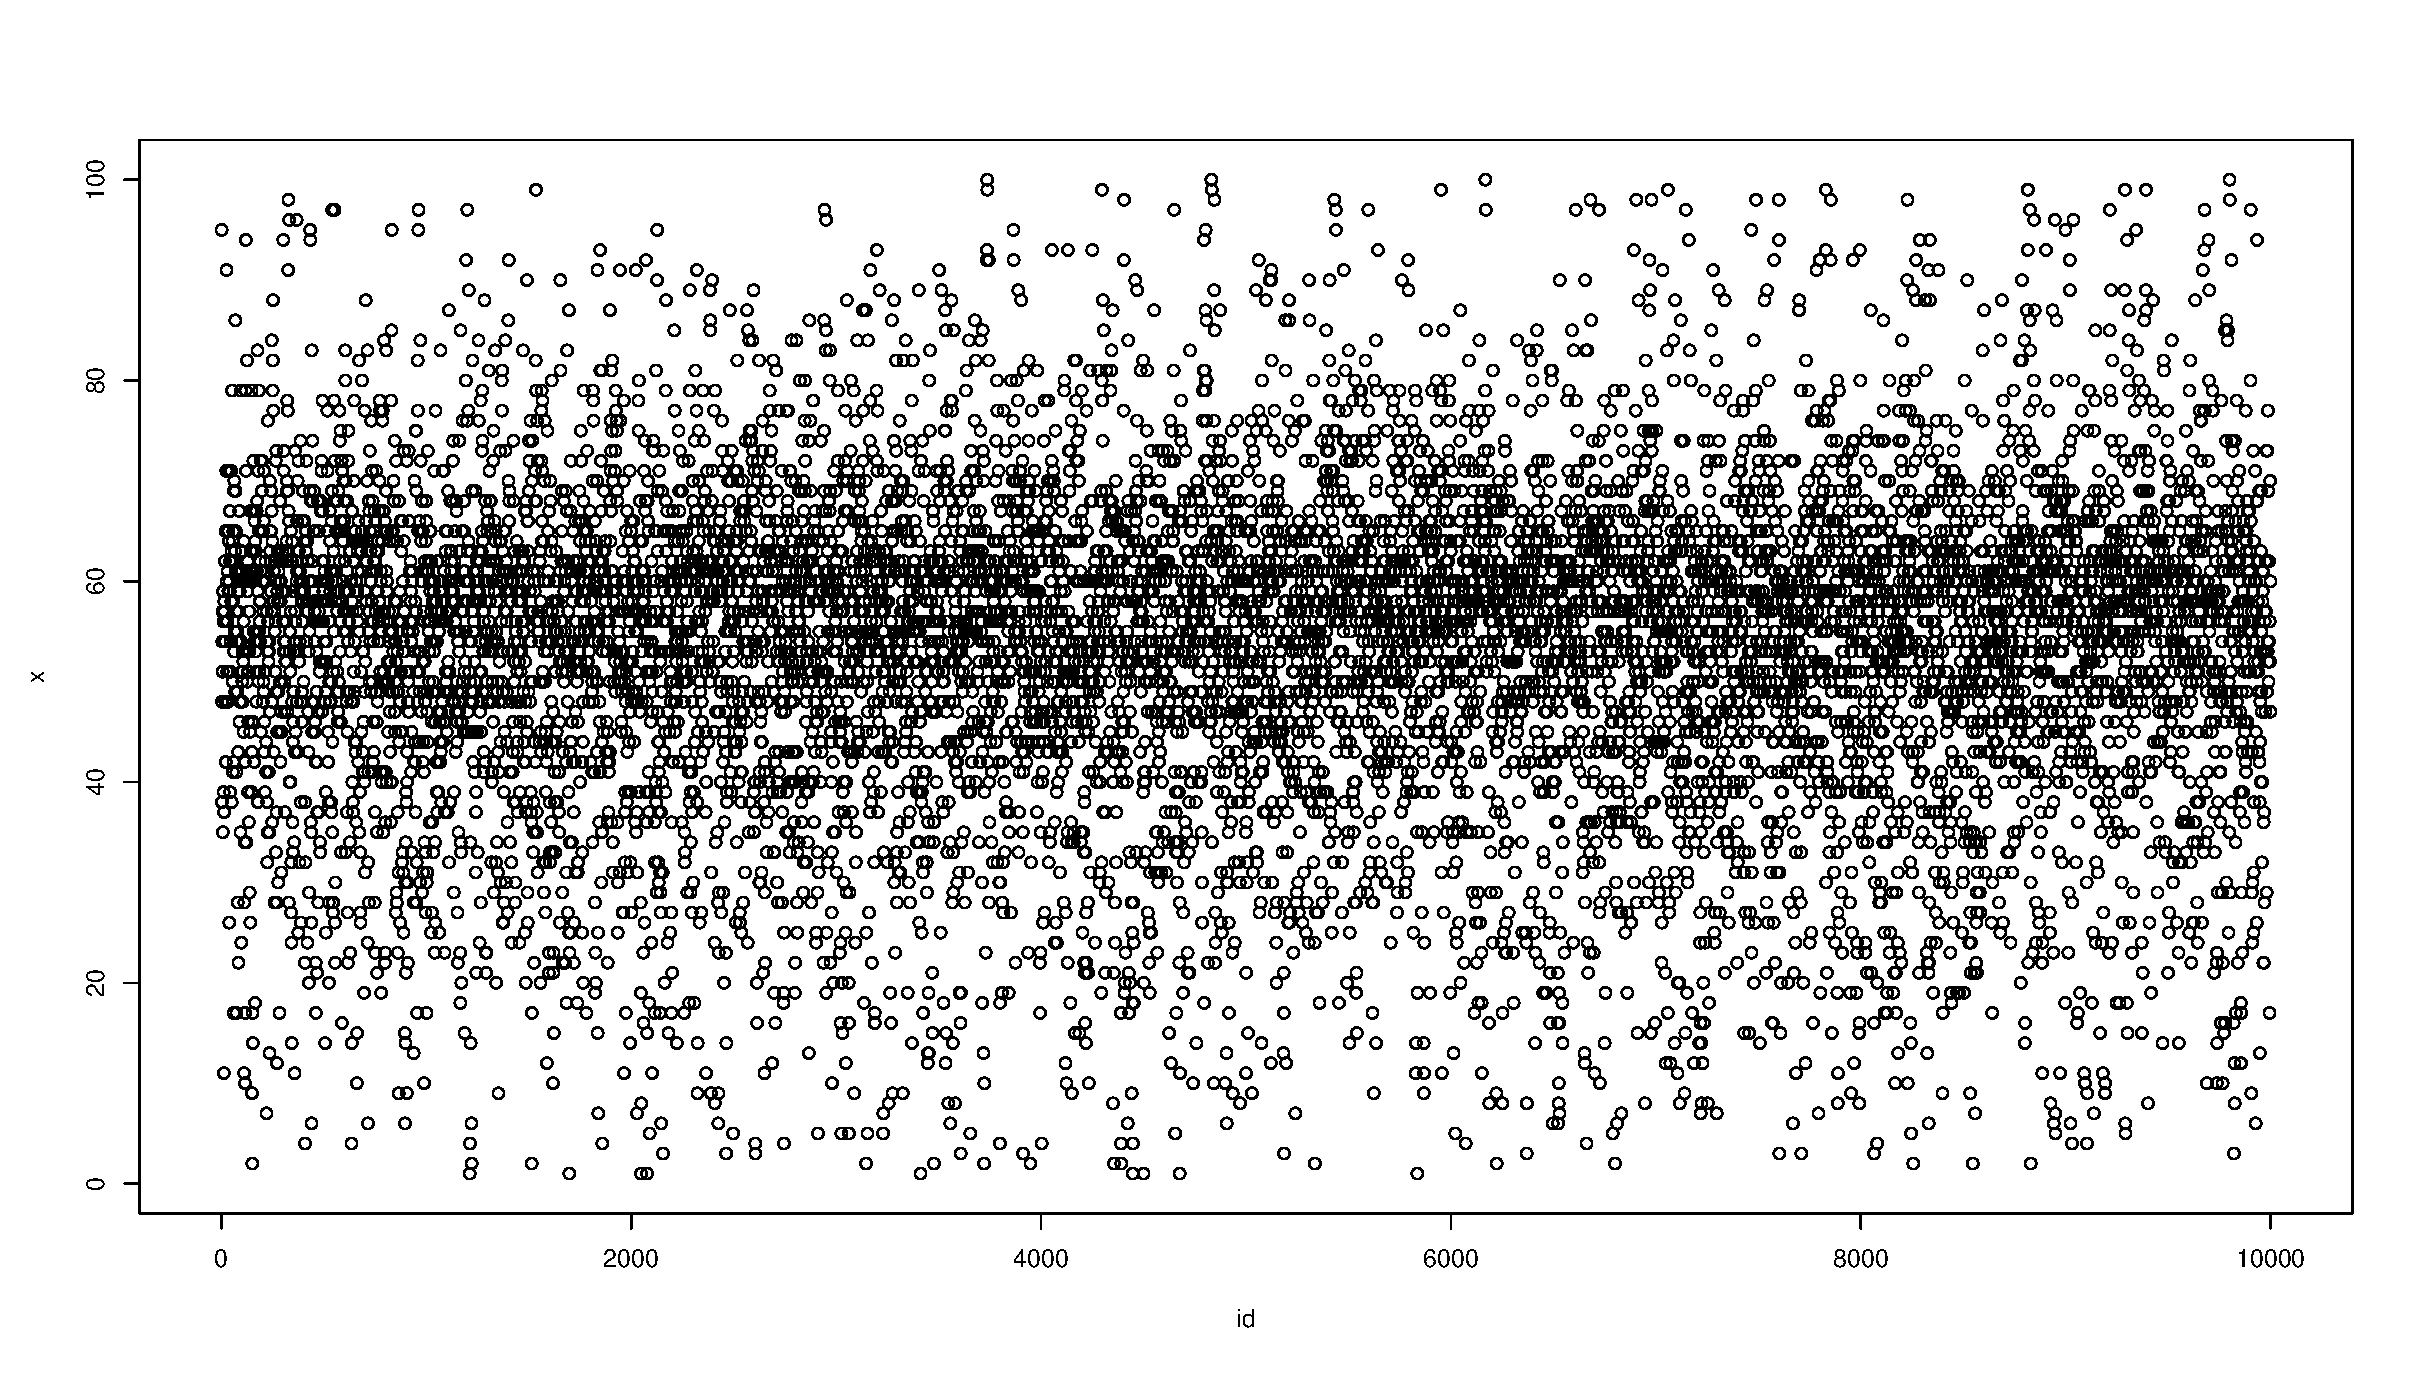
\includegraphics[width=5in]{sampling_n.eps}
\end{figure}

\begin{figure}
\caption{Sampling of $\lambda_1$}
\centering
	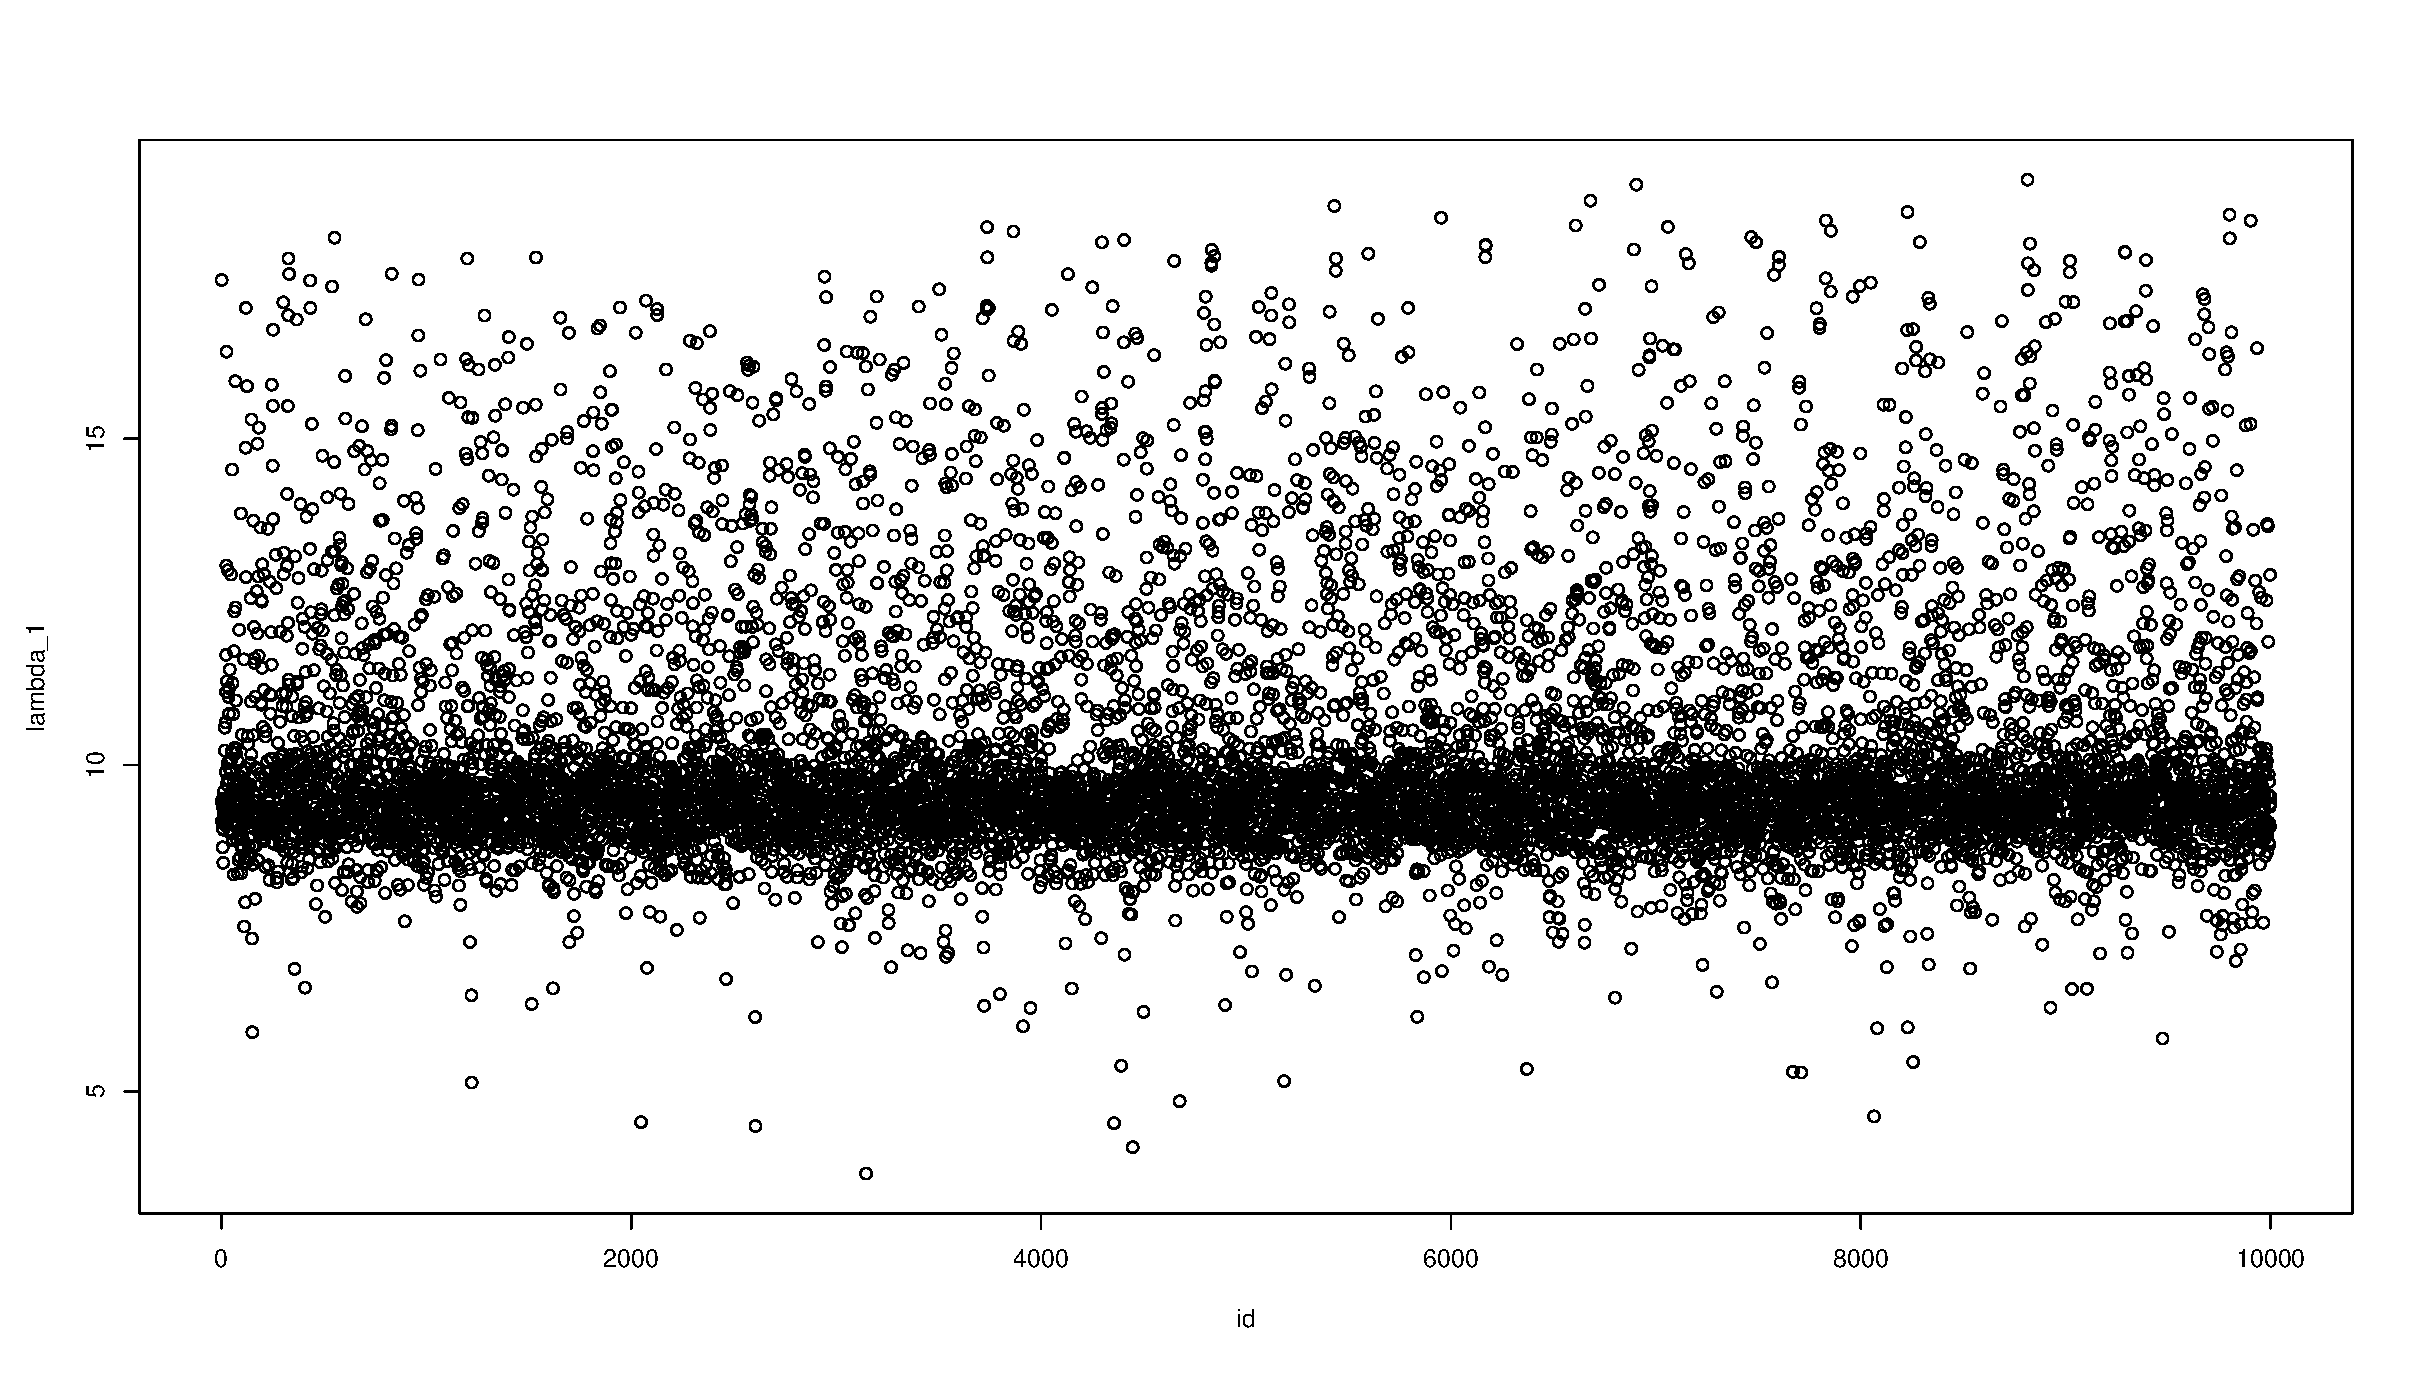
\includegraphics[width=5in]{sampling_lbd1.eps}
\end{figure}

\begin{figure}
\caption{Sampling of $\lambda_2$}
\centering
	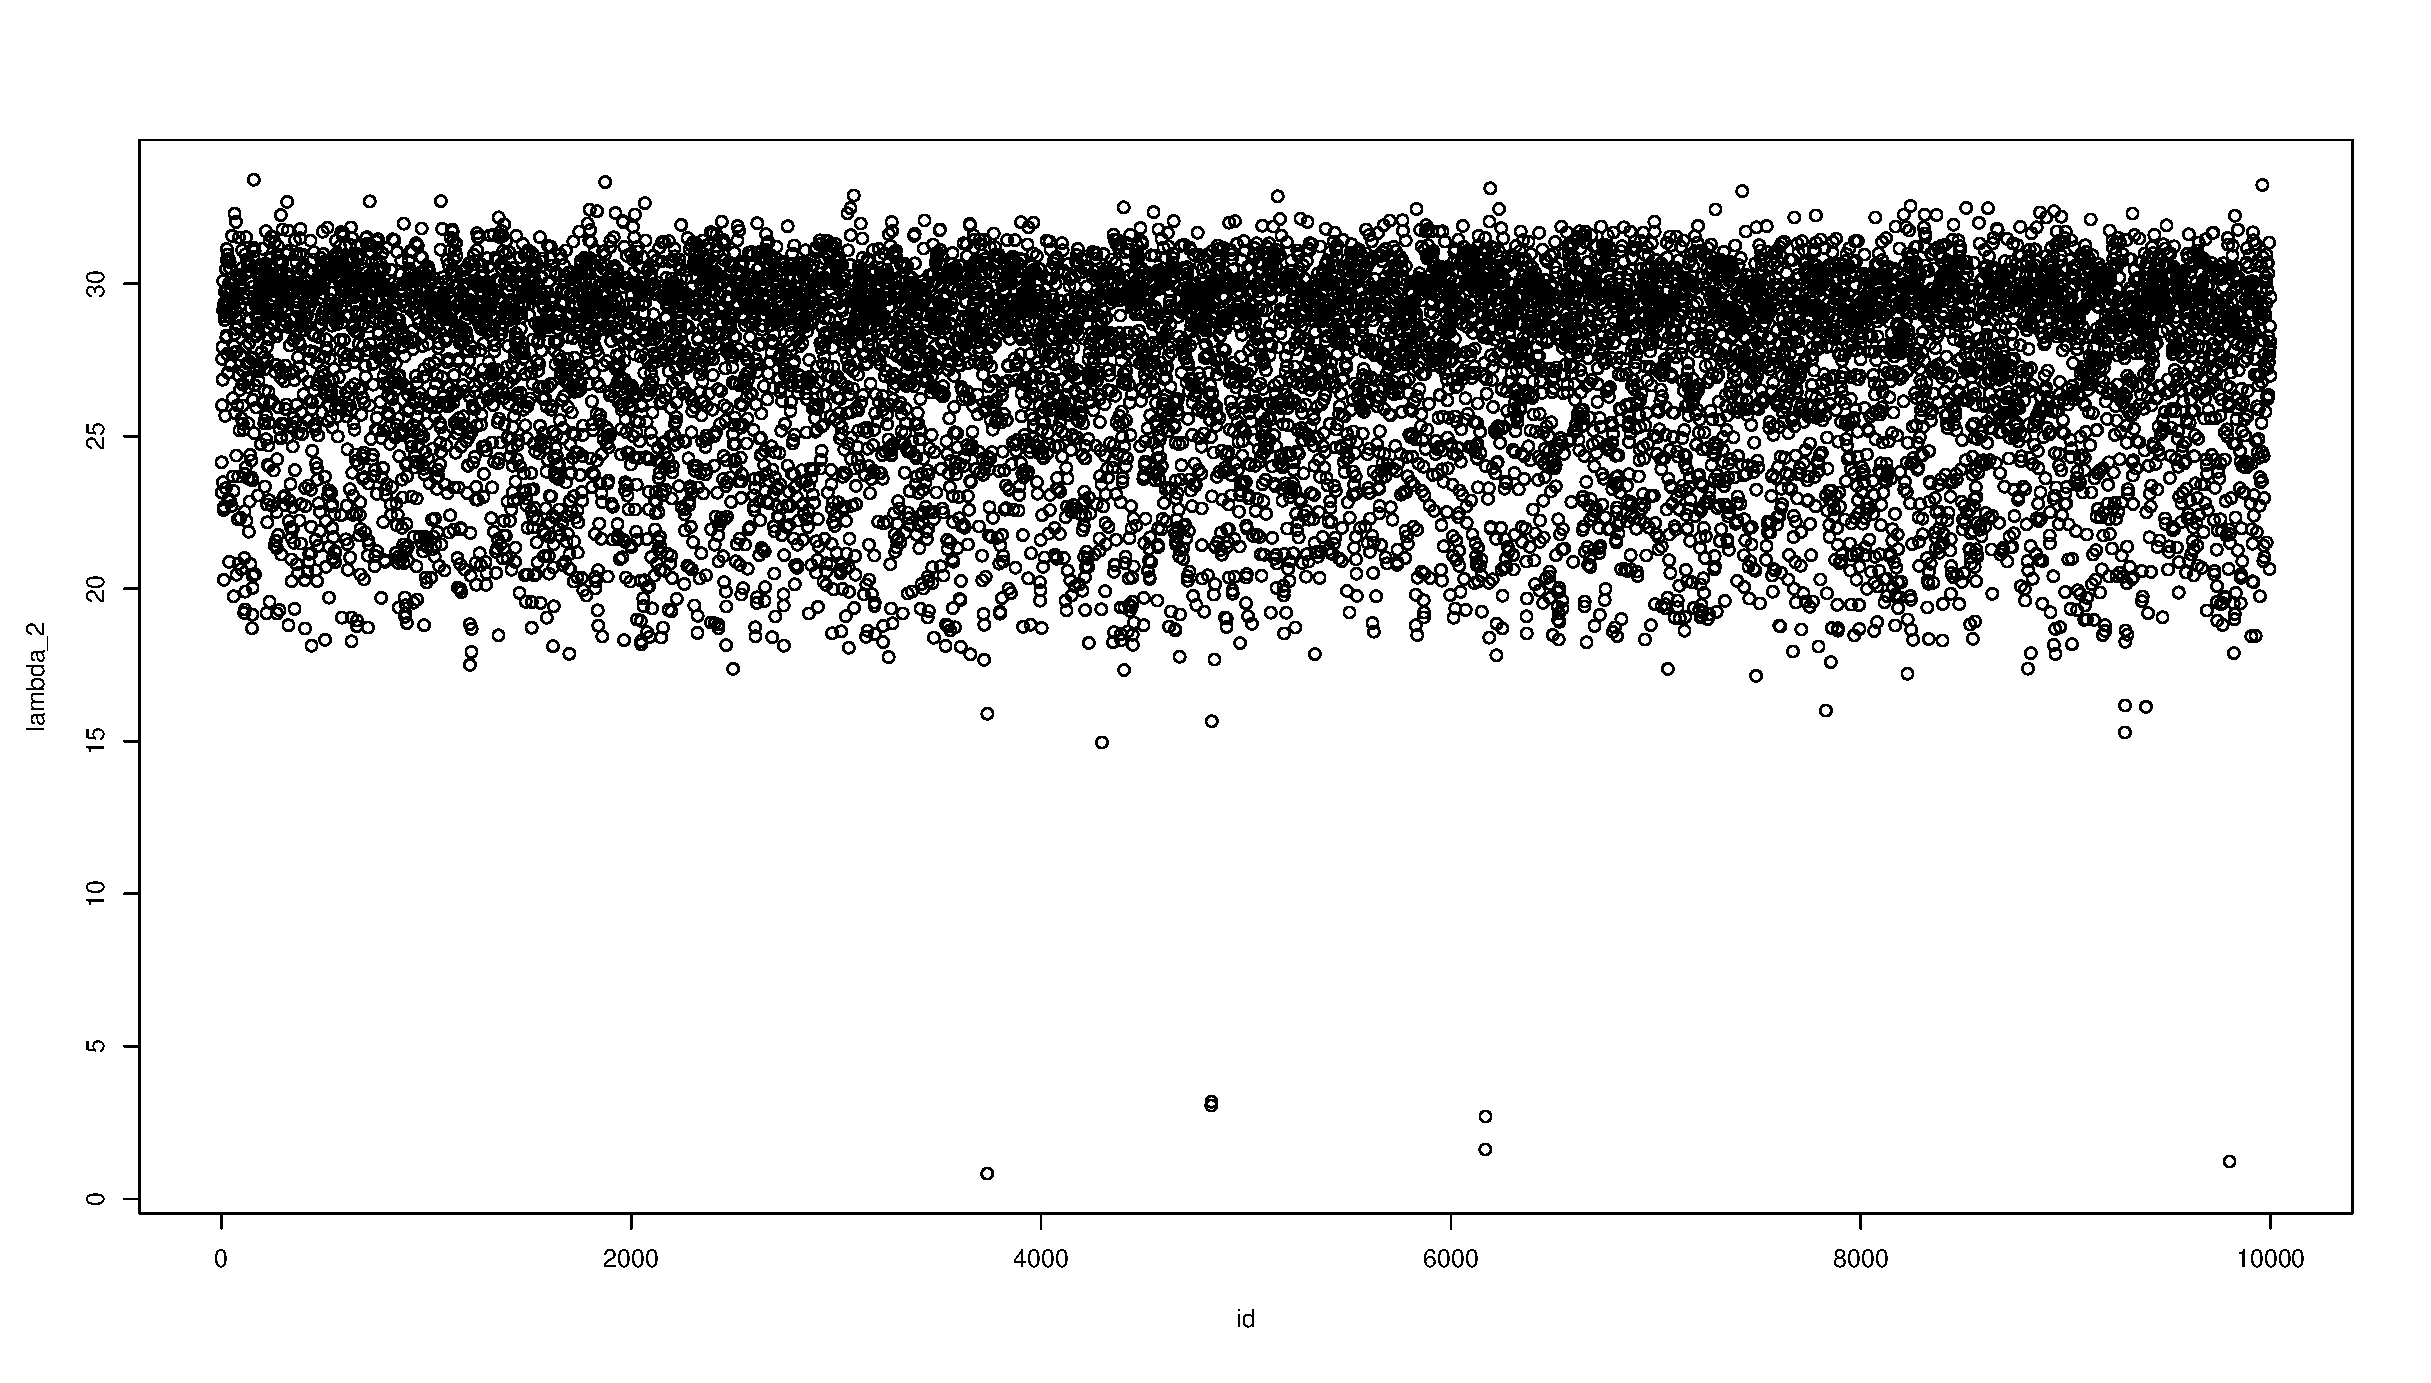
\includegraphics[width=5in]{sampling_lbd2.eps}
\end{figure}


\bibliographystyle{apalike}
\bibliography{bib}

\end{document}
